\section[Разработка структуры БД]{РАЗРАБОТКА СТРУКТУРЫ БАЗЫ ДАННЫХ}
\label{sect:db_structure}

В данном разделе рассматривается процесс проектирования разрабатываемого
интернет-магазина.

В подразделе~\ref{sub:db_structure_theory} даны фундаментальные определения теории
баз данных, необходимые для понимания излагаемого далее материала.

Далее, в подразделах~\ref{sub:db_structure_aims}~и~\ref{sub:db_structure_stages}
приведены цели, задачи, основные этапы проектирования баз данных.
В подразделах~\ref{sub:db_structure_concept_design},
\ref{sub:db_structure_logical_design}~и~\ref{sub:db_structure_physical_design}
подробно раскрыт каждый из этапов проектирования баз данных.

В процессе проектирования базы данных использовалось средство автоматизированного
проектирования CA ERWin.
Для построения диаграммы прецедентов было использовано CASE-средство
Enterprise Architect, разработанное компанией Sparx Systems.

\subsection{Основные определения}
\label{sub:db_structure_theory}

\textit{База данных} --- совместно используемый набор логически связанных данных
(и описание этих данных), предназначенный для удовлетворения информационных
потребностей организации.

\textit{Система управления базами данных (СУБД)} --- программное обеспечение,
с помощью которого пользователи могут определять, создавать и поддерживать базу данных,
а также осуществлять к ней контролируемый доступ~\cite{konnolli03}.

\textit{Модель данных} --- это абстрактное, самодостаточное,
логическое определение объектов, операторов и прочих элементов,
в совокупности составляющих абстрактную  машину доступа к данным,
с которой взаимодействует пользователь.

\textit{Реляционная модель данных} состоит из трех частей:
\begin{itemize}
\item
  \textit{структурная часть} описывает, какие объекты рассматриваются
  реляционной моделью. Единственной структурой данных, используемой
  в реляционной модели, являются \textit{нормализованные отношения}.
\item
  \textit{целостная часть} описывает ограничения специального вида,
  которые должны выполняться для любых отношений в любых реляционных базах данных.
  Это целостность сущностей и целостность внешних ключей.
\item
  \textit{манипуляционная часть} описывает два эквивалентных способа
  манипулирования реляционными данными --- \textit{реляционную алгебру} и
  \textit{реляционное исчисление}.
\end{itemize}

Процесс преобразования отношений базы данных к виду, отвечающему нормальным формам,
называется \textit{нормализацией}.

Переменная отношения находится в \textit{первой нормальной форме} тогда и только
тогда, когда в любом допустимом значении этой переменной отношения каждый её кортеж
содержит только одно значение для каждого из атрибутов.

Переменная отношения находится во \textit{второй нормальной форме} тогда и только тогда,
когда она находится в первой нормальной форме и каждый неключевой атрибут
неприводимо зависит от ее первичного ключа.

Переменная отношения находится в \textit{третьей нормальной форме} тогда и только
тогда, когда она находится во второй нормальной форме и в ней отсутствуют транзитивные
зависимости~\cite{date05}.

Переменная отношения находится в \textit{нормальной форме Бойса-Кодда} тогда и только тогда,
когда каждый её детерминант является потенциальным ключом~\cite{konnolli03}.

Необходимо отметить, что существуют нормальные формы более высоких порядков, но
на практике они используются реже.

*** аномалии ***

\subsection{Цели и задачи проектирования базы данных}
\label{sub:db_structure_aims}

Основные \textit{цели проектирования баз данных:}
\begin{itemize}
  \item централизация данных;
  \item сокращение избыточности и дублирования данных;
  \item обеспечение целостности БД;
  \item обеспечение возможности получения данных по всем необходимым запросам.
\end{itemize}

\textit{Задача проектирования базы данных} в общем случае формулируется следующим образом: выбрать
подходящую структуру для заданного массива данных, которое требуется поместить в базу данных.
Иначе говоря, нужно решить вопрос, какие необходимы базовые переменные отношения и какой
набор атрибутов они должны включать~\cite{date05}.

\subsection{Этапы проектирования баз данных}
\label{sub:db_structure_stages}
В общем случае выделяют три этапа проектирования баз данных:
\begin{itemize}
  \item концептуальное проектирование;
  \item логическое проектирование;
  \item физическое проектирование.
\end{itemize}

\pagebreak

Рассмотрим каждый из этапов подробнее.

\textit{Концептуальное (инфологическое) проектирование} --- создание концептуального
представления базы данных, включающее определение типов важнейших сущностей и существующих
между ними связей и атрибутов.

Концептуальное проектирование базы данных начинается с создания концептуальной
модели данных предприятия, полностью независимой от любых деталей
реализации.
К последним относятся выбранный тип СУБД,
состав программ приложения, используемый язык программирования, конкретная аппаратная
платформа, вопросы производительности и любые другие физические особенности реализации.


\textit{Логическое (даталогическое) проектирование} --- преобразование
концептульного представления в логическую структуру базы данных,
включая проектирование отношений.

Логическое проектирование базы данных заключается в преобразовании
концептуальной модели данных в логическую модель данных предприятия с учетом
выбранного типа СУБД (например, предполагается использование
реляционной СУБД). Логическая модель данных является источником информации
для этапа физического проектирования. Она предоставляет разработчику
физической модели данных средства проведения всестороннего анализа различных
аспектов работы с данными, что имеет исключительно важное значение для
выбора действительно эффективного проектного решения.

\textit{Физическое проектирование} --- принятие решения о том, как логическая модель
будет физически реализована (с помощью таблиц) в базе данных, создаваемой
с использованием выбранной СУБД.

Физическое проектирование базы данных предусматривает принятие разработчиком
окончательного решения о способах реализации создаваемой базы. Поэтому
физическое проектирование обязательно производится с учетом всех особенностей
используемой СУБД. Между этапами физического и логического проектирования
всегда имеется определенная обратная связь, поскольку решения,
принятые на этапе физического проектирования с целью повышения производительности
разрабатываемой системы, могут потребовать определенной корректировки логической
модели данных~\cite{konnolli03}.

\subsection{Концептуальное проектирование}
\label{sub:db_structure_concept_design}

\paragraph{}
Разрабатываемый интернет-магазин должен предоставлять актуальную информацию о
имеющихся в продаже товарах конечному пользователю, позволять совершать покупки.

Так, \textit{пользователь} имеет возможность просматривать все веб-страницы,
совершать покупки, а также экспортировать данные о товарах в файлы формата xml.

\textit{Администратор} разрабатываемого интернет-магазина просматривает
и редактирует каталог товаров. Также он имеет возможность
пополнения каталога товаров путём загрузки информации в базу данных с
локального носителя.

На рисунке~\ref{fig:use_case} изображена диаграмма прецедентов
разрабатываемого интернет-магазина.

\begin{figure}[h]
  \centering
  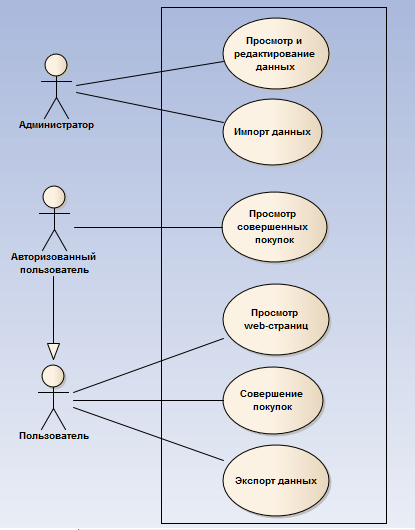
\includegraphics[width=130mm]{pic/use_case.png}
  \caption{Диаграмма прецедентов \\ проектируемого интернет-магазина}
  \label{fig:use_case}
\end{figure}

\paragraph{}
Пополнение каталога товаров разрабатываемого интернет-магазина должно осуществляться
только администратором путём использования веб-интерфейса разрабатываемого
интернет-магазина, или путём загрузки информации
о товарах напрямую в базу данных используя файлы с расширением xml.

\paragraph{}
Исходя из описанных выше минимальных требований к разрабатываемой
системе, можно выделить следующие необходимые объекты-сущности:
\begin{itemize}
  \item <<велосипеды>> --- хранит полное описание велосипеда;
  \item <<велотовары>> --- хранит полное описание велотовара;
  \item <<товары в наличии>> --- хранит информацию о товарах, находящихся в наличии;
  \item <<заказы товаров>> --- хранит информацию о заказах, ожидающих выполнения;
  \item <<архив заказов>> --- сохраняет информацию о совершенных пользователями
    покупках;
  \item <<пользователи>> --- хранит информацию о зарегистрированных
    в системе пользователях.
\end{itemize}

На рисунке~\ref{fig:ER_model} представлена ER-модель
разрабатываемого интернет-магазина.

\begin{figure}[h]
  \centering
  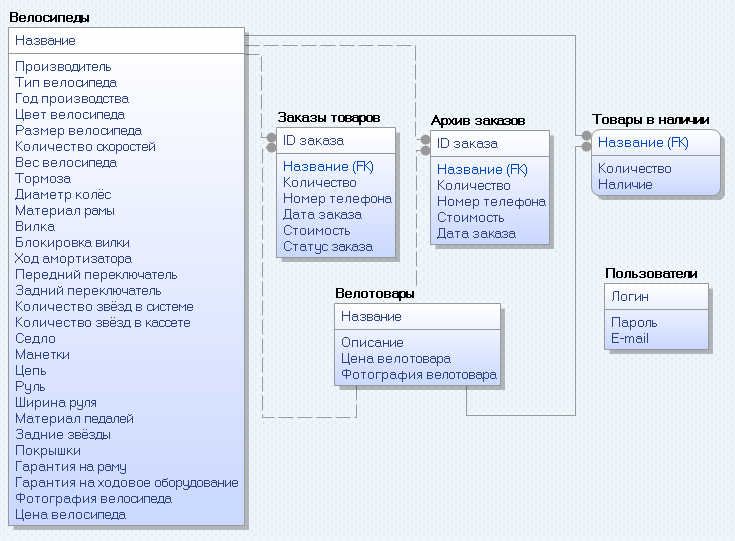
\includegraphics[width=165mm]{pic/ER.png}
  \caption{ER-модель проектируемого интернет-магазина}
  \label{fig:ER_model}
\end{figure}

*** рассмотреть некоторые сущности подробнее ***


\subsection{Логическое проектирование}
\label{sub:db_structure_logical_design}

\subsection{Физическое проектирование}
\label{sub:db_structure_physical_design}



\pagebreak
